%%%%%%%%%%%%%%%%%%%%%%%%%%%%%%%%%%%%%%%%%%%%%%%%%%%%%%%%%%%%%%%%%%%%%%%%%%%%%%%
%                         File: osa-revtex4-1.tex                             %
%                        Date: April 15, 2013                                 %
%                                                                             %
%                              BETA VERSION!                                  %
%                   JOSA A, JOSA B, Applied Optics, Optics Letters            %
%                                                                             %
%            This file requires the substyle file osajnl4-1.rtx,              %
%                   running under REVTeX 4.1 and LaTeX 2e                     %
%                                                                             %
%                   USE THE FOLLOWING REVTeX 4-1 OPTIONS:                     %
% \documentclass[osajnl,twocolumn,showpacs,superscriptaddress,10pt]{revtex4-1}%
%                    %% Use 11pt for Applied Optics                           %
%                                                                             %
%               (c) 2013 The Optical Society of America                       %
%                                                                             %
%%%%%%%%%%%%%%%%%%%%%%%%%%%%%%%%%%%%%%%%%%%%%%%%%%%%%%%%%%%%%%%%%%%%%%%%%%%%%%%

\documentclass[osajnl,twocolumn,showpacs,superscriptaddress,10pt]{revtex4-1} %% use 11pt for Applied Optics
%%\documentclass[osajnl,preprint,showpacs,superscriptaddress,12pt]{revtex4-1} %% use 12pt for preprint option
\usepackage{amsmath,amssymb,graphicx,float}
\usepackage[utf8]{inputenc}
\graphicspath{ {images/} }

\begin{document}

\title{SGEMM GPU kernel performance Data Set}

\author{Ulises Jeremias Cornejo Fandos}
\affiliation{Licenciatura en Informatica - 13566/7, Facultad de Informatica, UNLP}

\author{Gaston Gustavo Rios}
\affiliation{Licenciatura en Informatica - 13591/9, Facultad de Informatica, UNLP}


\begin{abstract}
Resumen
\end{abstract}

\maketitle %% required

\section{Introducción}

\subsection{SGEMM GPU kernel performance Data Set}

El conjunto de datos a analizar mide el tiempo de ejecución, \textit{en milisegundos}, de un producto matriz-matriz $A * B = C$, donde las matrices tienen un tamaño de $2048 x 2048$, usando un núcleo de \textit{GPU SGEMM} parametrizable con \textit{241600} posibles combinaciones de parámetros. Para cada combinación probada, se realizan 4 corridas y sus resultados se disponen en las ultimas 4 columnas. \\

Hay 14 parámetros, los primeros 10 son ordinales y solo pueden tomar hasta 4 potencias diferentes de dos valores, y las 4 últimas variables son binarias. De las 1327104 combinaciones de parámetros totales, solo 241600 son factibles \textit{(debido a varias restricciones del kernel)}. Este conjunto de datos contiene los resultados de todas estas combinaciones posibles. \\

El experimento se ejecutó en una estación de trabajo de escritorio que ejecuta Ubuntu 16.04 Linux con un Intel Core i5 (3.5GHz), 16GB de RAM y una NVidia Geforce GTX 680 4GB GF580 GTX-1.5GB GPU. Se utiliza el kernel \textit{gemm\_fast} de la biblioteca de sintonización de kernel automática de OpenCL 'CLTune'. \\

\subsubsection{}{Información de los atributos}

\begin{itemize}
    \item \textbf{Variables independientes}

    \begin{itemize}
        \item \textit{1-2. $M_{wg}$, $N_{wg}$:} bloque 2D por matriz a nivel de grupo de trabajo. Toma valores enteros del conjunto $\{16, 32, 64, 128\}$.
        \item \textit{3. $K_{wg}$:} dimesión interna del bloque 2D a nivel de grupo de trabajo. Toma valores enteros del conjunto $\{16, 32\}$.
        \item \textit{4-5. $M_{dim}C$, $N_{dim}C$:} tamaño del grupo de trabajo local. Toma valores enteros del conjunto $\{8, 16, 32\}$.
        \item \textit{6-7. $M_{dim}A$, $N_{dim}B$:} forma de la memoria local. Toma valores enteros del conjunto $\{8, 16, 32\}$.
        \item \textit{8. $K_{wi}$:} factor de desenrollado del bucle del kernel. Toma valores enteros del conjunto $\{2, 8\}$.
        \item \textit{9-10. $V_{wm}$, $V_{wn}$:} anchos de vectores por matriz para cargar y almacenar. Toma valores enteros del conjunto $\{1, 2, 4, 8\}$.
        \item \textit{11-12. $M_{stride}$, $N_{stride}$:} stride habilitado para acceder a la memoria off-chip en un único hilo. Variable binaria.
        \item \textit{13-14. $S_{A}$, $S_{B}$:} Almacenamiento en caché manual por matriz del mosaico del grupo de trabajo 2D. Variable binaria.
    \end{itemize}

    \begin{itemize}
        \item \textit{15-18. $Run_1$, $Run_2$, $Run_3$, $Run_4$:} tiempos de rendimiento en milisegundos para 4 ejecuciones independientes con los mismos parámetros. Toman valores reales del intervalo $[13.25, 3397.08]$.
    \end{itemize}
\end{itemize}

\subsection{Conjunto de datos a analizar}

Para decidir las tecnologías y conjunto de datos a utilizar se evalúan distintas posibilidades intentardo así optar por la que mejor se adapte a las necesidades y dominio del problema. \\

Como se muestra en la sub-sección anterior, el conjunto de datos planteado dispone de una gran cantidad de ejemplos \textit{(241600 combinaciones de parámetros)}. Para realizar el análisis sobre este conjunto de datos, se busca utilizar un software el cual permite el análisis de hasta 10000 ejemplos, por lo que se reduce el tamaño del espacio muestral a utilizar buscando no perder información relevante para el dominio del problema. \\

Para esto se decide que sería conveniente evaluar cuáles de esos parámetros son más relevantes y, a su vez, cuáles de los valores tomados por cada uno generan cambios reales en los tiempos de ejecución resultante. Para esto se limita esta evaluación a aquellos parámetros cuyos posibles valores pertenezcan a un conjunto de cardinalidad mayor que dos, dado que así presentan más configuraciones posibles. \\

Se toman los parámetros $M_{wg}$ y $N_wg$ solo las filas que tienen valores pertenecientes a ${64, 128}$, quedando así la mitad de ejemplos. Esta cantidad se puede reducir más fijando alguno de los parámetros, lo cual sería muy conveniente. Luego, se observa que en dos de los datos categóricos, la configuración más eficiente es $(S_{A}, S_{B}) = (1, 1)$. De esto surge la duda de si podrían quitarse los casos en los que uno de ellos, o ambos, sean “no”. Se considera que con esto podría reducirse lo suficiente para poder así procesar los datos. Y finalmente tenemos que buscar cómo podemos dividirlo en dos datasets. \\

Aplicando dichas reducciones se ve que con el conjunto de datos resultante pierde mucha información potencialmente valiosa. Es por esto que se decide evaluar nuevas posibilidades llegando así a la opción utilizada. \\

Se opta por analizar y construir modelos de sistemas inteligentes evaluando la totalidad de los datos utilizando nuevas tecnologías de las cuales se detalla más en la siguientes subsecciones. \\

El conjunto de datos permanece intacto comparado con el original a diferencia de las columnas de tiempo de ejecución que se descartan luego de generar un único atributo el cual sea igual a la media de los 4 anteriores. \\

\section{Marco Teórico}

En esta sección se introduce brevemente conceptos básicos necesarios para abordar los contenidos de las siguientes secciones del informe con mayores referencias y capacidad de entendimiento. \\

\subsection{Clustering}

Un algoritmo de agrupamiento (en inglés, clustering) es un procedimiento de agrupación de una serie de vectores de acuerdo con un criterio. Esos criterios son por lo general distancia o similitud. La cercanía se define en términos de una determinada función de distancia, como la euclídea, aunque existen otras más robustas o que permiten extenderla a variables discretas. La medida más utilizada para medir la similitud entre los casos es la matriz de correlación entre los nxn casos. Sin embargo, también existen muchos algoritmos que se basan en la maximización de una propiedad estadística llamada verosimilitud. \\

En el contexto de la Mineria de Datos se lo considera una técnica de aprendizaje no supervisado puesto que busca encontrar relaciones entre variables descriptivas pero no la que guardan con respecto a una variable objetivo. \\

\subsubsection{K-Means}

\textbf{K-means} es un método de agrupamiento, que tiene como objetivo la partición de un conjunto de n observaciones en k grupos en el que cada observación pertenece al grupo cuyo valor medio es más cercano. \\

En la figura \ref{figure:clustering_example} se muestra un ejemplo de aplicación del algoritmo k-means para realizar un agrupamiento de los datos.

\begin{figure}[H]
    \centering
    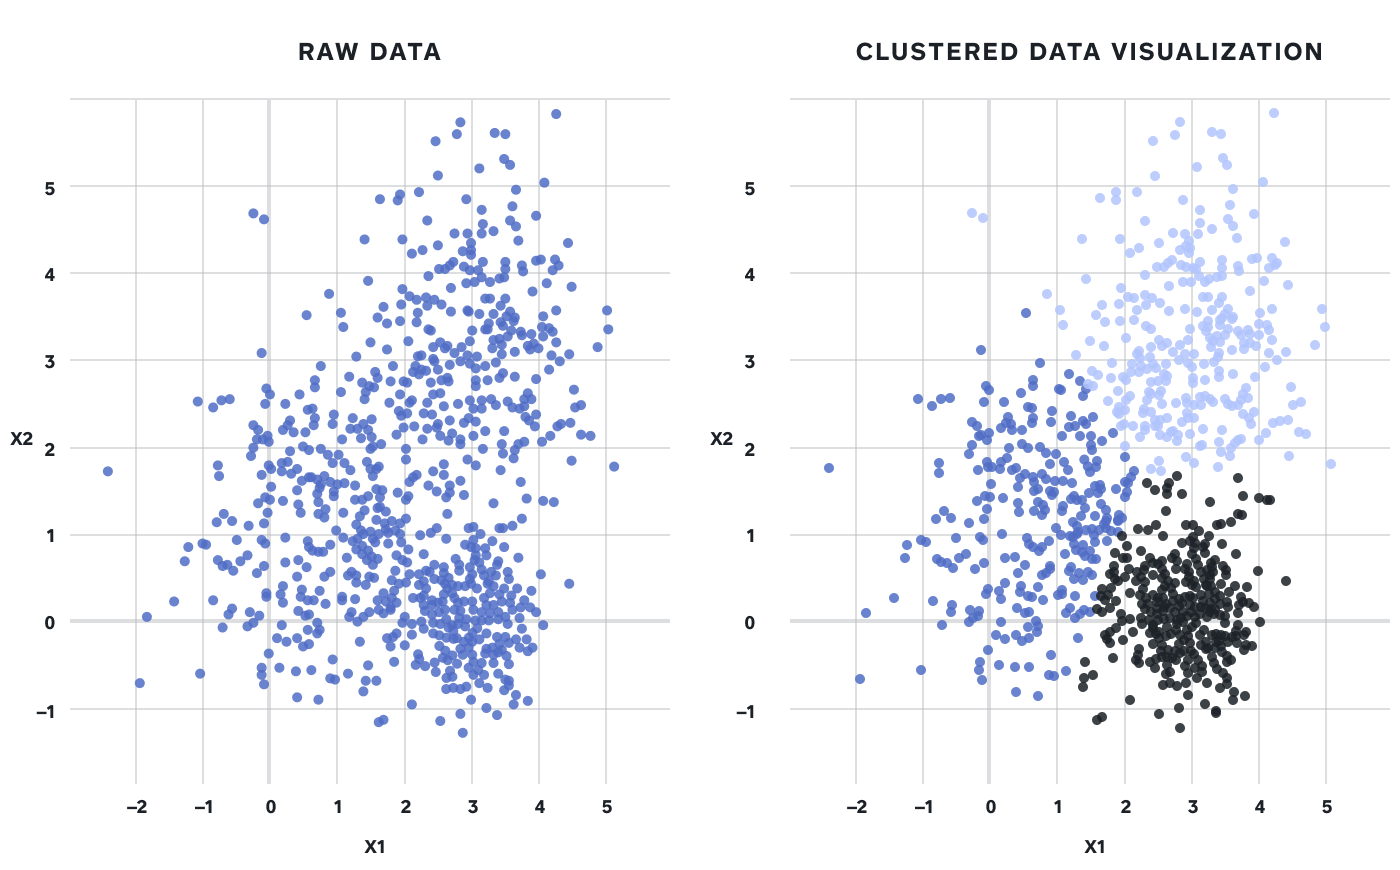
\includegraphics[width=0.4\textwidth]{theory/clustering}
    \caption{Ejemplo de aplicación del algoritmo k-means para realizar un agrupamiento de los datos.}
    \label{figure:clustering_example}
\end{figure}

\subsection{Redes Neuronales}

Las \textbf{redes neuronales} son un modelo computacional basado en un gran conjunto de unidades neuronales simples, \textbf{neuronas artificiales}, de forma aproximadamente análoga al comportamiento observado en los axones de las neuronas en los cerebros biológicos. \\

Cada unidad neuronal está conectada con muchas otras y los enlaces entre ellas pueden incrementar o inhibir el estado de activación de las neuronas adyacentes. Cada unidad neuronal, de forma individual, opera empleando funciones de suma. Puede existir una función limitadora o umbral en cada conexión y en la propia unidad, de tal modo que la señal debe sobrepasar un límite antes de propagarse a otra neurona. \\

Estos sistemas aprenden y se forman a sí mismos, en lugar de ser programados de forma explícita, y sobresalen en áreas donde la detección de soluciones o características es difícil de expresar con la programación convencional.

\subsubsection{Perceptron}

En el campo de las Redes Neuronales, el \textbf{perceptrón}, se refiere a la neurona artificial o unidad básica de inferencia en forma de discriminador lineal, a partir del cual se desarrolla un algoritmo capaz de generar un criterio para seleccionar un sub-grupo a partir de un grupo de componentes más grande. \\

En la figura \ref{figure:perceptron_example} se muestra la arquitectura que determina el comportamiento de un perceptron.

\begin{figure}[H]
    \centering
    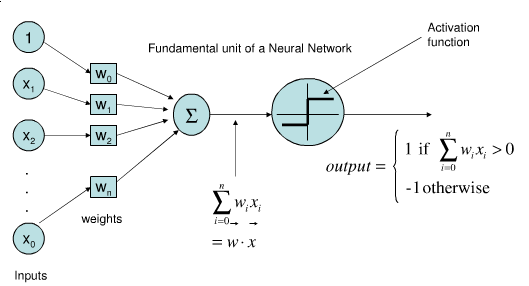
\includegraphics[width=0.4\textwidth]{theory/perceptron}
    \caption{Arquitectura de un perceptron.}
    \label{figure:perceptron_example}
\end{figure}

La limitación de este algoritmo es que si dibujamos en un gráfico estos elementos, se deben poder separar con un hiperplano únicamente los elementos "deseados" discriminándolos (ó \textit{separándolos}) de los \textit{"no deseados"} como se muestra en la figura \ref{figure:linear_example}.

\begin{figure}[H]
    \centering
    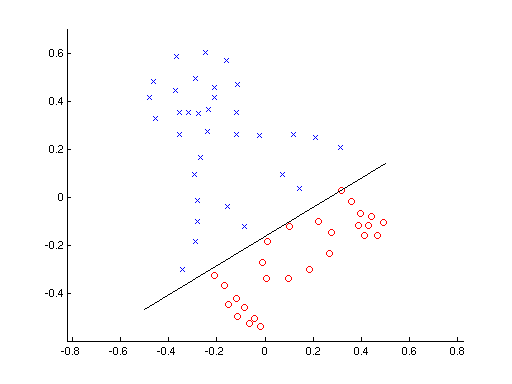
\includegraphics[width=0.4\textwidth]{theory/linear}
    \caption{Ejemplo de función linear discriminante.}
    \label{figure:linear_example}
\end{figure}

El perceptrón puede utilizarse con otros tipos de perceptrones o de neurona artificial, para formar una red neuronal artificial más compleja.

\subsubsection{Multiperceptrón}

El \textbf{perceptrón multicapa}, \textit{multi-perceptrón}, es una red neuronal artificial formada por múltiples capas, de tal manera que tiene capacidad para resolver problemas que no son linealmente separables que, como se explica en la subsección anterior, es la principal limitación del \textit{perceptrón}. El perceptrón multicapa puede estar totalmente o localmente conectado. En el primer caso cada salida de una neurona de la capa \textit{"i"} es entrada de todas las neuronas de la capa \textit{"i+1"}, mientras que en el segundo cada neurona de la capa \textit{"i"} es entrada de una serie de neuronas (región) de la capa \textit{"i+1"}. \\

Se muestra en la figura (\ref{figure:multiperceptron_example}) un ejemplo de la arquitectura de un perceptron multicapa.

\begin{figure}[H]
    \centering
    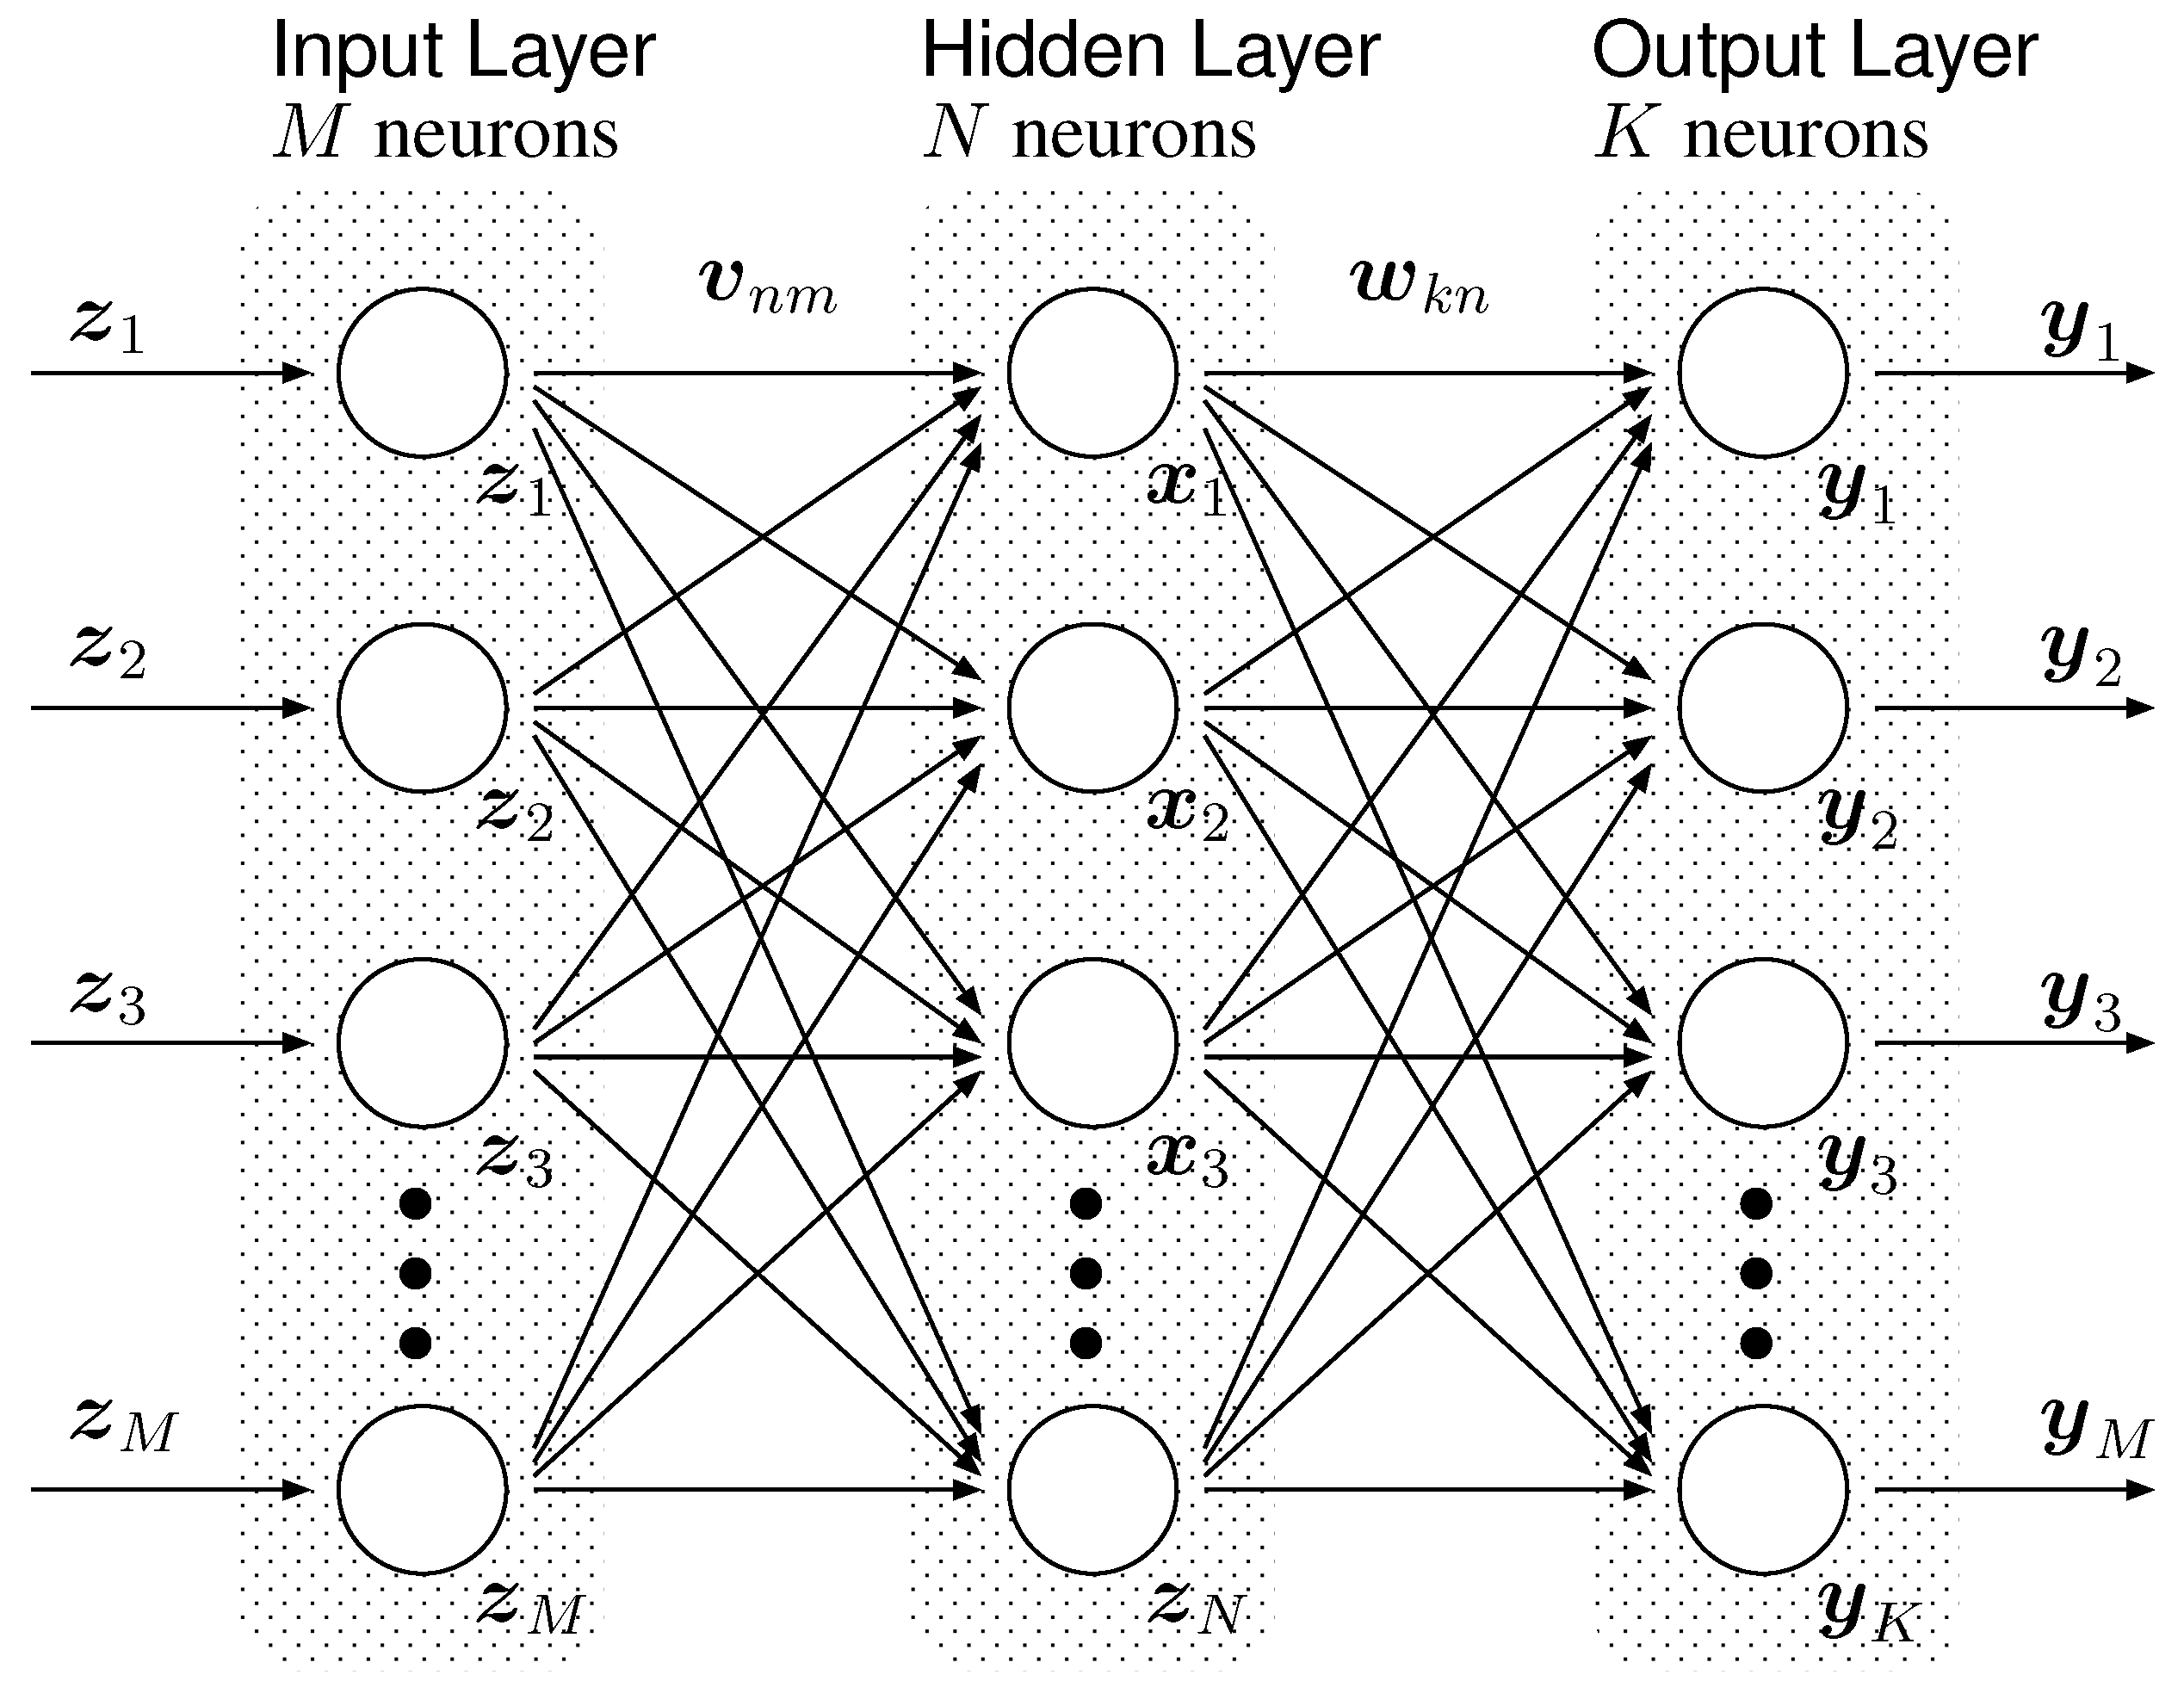
\includegraphics[width=0.4\textwidth]{theory/multiperceptron}
    \caption{Ejemplo básico de un multiperceptron.}
    \label{figure:multiperceptron_example}
\end{figure}

\section{Análisis de datos}

Para el análisis de los datos se evalúan distintas gráficas de lo mismos, como histogramas de los datos nominales y gráficas de dispersión para aquellos datos de tipo numérico, además de ciertas métricas que permiten conocer la correlación entre cada uno de ellos. De este modo se permite observar relaciones entre los distintos atributos del conjunto de datos así como también la relación entre estos mismos y la etiqueta, o \textit{label}.

\begin{flushright}
\textit{\footnotesize Se dispone de las gráficas correspondientes a los atributos en la sección \ref{apendix:images:attr} del apéndice.}
\end{flushright}

\section{Método Experimental}

En esta sección se detalla todo lo referido al estudio y la creación de los distintos modelos de sistemas inteligentes utilizados para el estudio del conjunto de datos elegido. \\

Para el análisis de este dataset se utilizan dos modelos de sistemas inteligentes detallados a continuación.

\section{Clustering}

\subsection{K-Means}

Para la construcción de este modelo se utiliza el algoritmo K-means evaluando las distancias con distancia euclidea. Se evalúa la calidad del modelo resultante utilizando el índice de Silhouette notando que se obtienen mejores resultandos cuando el número de clusters $k$ es igual a 2, obteniendo finalmente un índice de Silhouette igual a 0.824. Una comparativa entre la cantidad de clusters y el indice de Silhouette obtenido se puede observar en la tabla (\ref{table:clusters_silhouette}). \\

\begin{table}[h!]
    \centering
    \begin{tabular}{ccccccc}
        centroides & tiempo & silhouette \\
        \hline
        2 & 1.60s	& 0.824 \\
        3 & 1.42s	& 0.749 \\
        4 & 3.19s	& 0.587 \\
        5 & 3.26s	& 0.512 \\
        6 & 2.43s	& 0.503 \\
        7 & 3.01s	& 0.538 \\
        8 & 3.33s	& 0.380 \\
        9 & 3.43s	& 0.396 \\
        \hline
    \end{tabular}
    \caption{Comparativa entre la cantidad de clusters y el indice de Silhouette obtenido}
    \label{table:clusters_silhouette}
\end{table}

Como resultado se obtienen dos agrupamientos, \textit{cluster\_0} y \textit{cluster\_1}. Se pueden ver los datos del agrupamiento en la tabla (\ref{table:k_means}).

\begin{table}[h!]
    \centering
    \begin{tabular}{|ccc|ccc|}
        \hline
        cluster & atributo & centroide & cluster & atributo & centroide \\
        \hline
        0	& MWG & 77.454 & 1 &	MWG & 116.948 \\
        0	& NWG & 77.428 & 1 &	NWG & 117.277 \\
        0	& KWG & 25.436 & 1 &	KWG & 26.465 \\
        0	& MDIMC & 14.294 & 1 &	MDIMC & 9.517 \\
        0	& NDIMC & 14.316 & 1 &	NDIMC & 9.241 \\
        0	& MDIMA & 17.385 & 1 &	MDIMA & 17.201 \\
        0	& NDIMB & 17.380 & 1 &	NDIMB & 17.265 \\
        0	& KWI & 4.955 & 1 &	KWI & 5.556 \\
        0	& VWM & 2.382 & 1 &	VWM & 3.266 \\
        0	& VWN & 2.387 & 1 &	VWN & 3.211 \\
        0	& STRM & 0.500 & 1 &	STRM & 0.502 \\
        0	& STRN & 0.500 & 1 &	STRN & 0.505 \\
        0	& SA & 0.482 & 1 &	SA & 0.723 \\
        0	& SB & 0.482 & 1 &	SB & 0.720 \\
        0	& Run & 132.668 & 1 &	Run & 1265.095 \\
        \hline
    \end{tabular}
    \caption{Resultados del clustering generado con k\_means}
    \label{table:k_means}
\end{table}

\begin{thebibliography}{99}
%% Do not include separate BibTeX files; if BibTeX is used,
%% paste the output (contents of .bbl file) here.

\bibitem{revtex-au} \url{https://authors.aps.org/revtex4/}.
\bibitem{osastyle} \url{http://www.opticsinfobase.org/submit/style/jrnls_style.cfm}.

\end{thebibliography}

\clearpage

\onecolumngrid

\section{Apéndice}

\subsection{Imágenes} \label{apendix:images}

\subsubsection{Gráficos de los atributos} \label{apendix:images:attr}

\twocolumngrid

\begin{figure}[H]
    \centering
    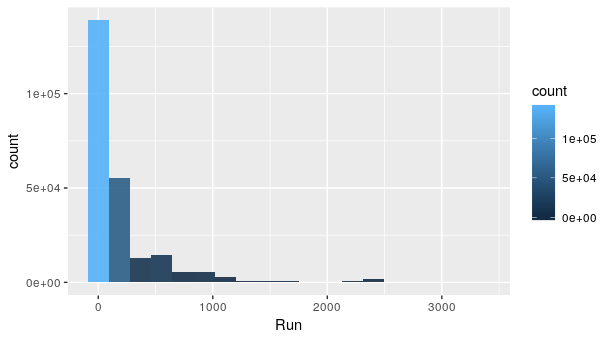
\includegraphics[width=0.45\textwidth]{plots/run_hist}
    \caption{Histograma del atributo Run.}
    \label{figure:run_hist}
\end{figure}

\begin{figure}[H]
    \centering
    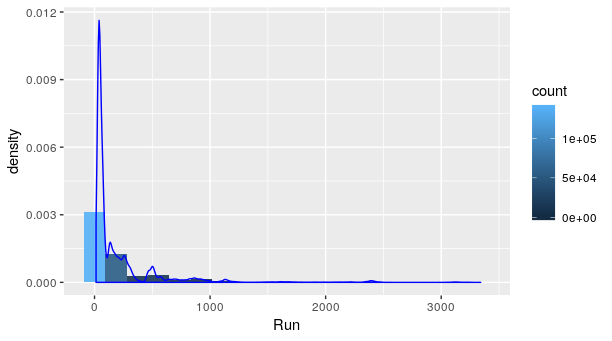
\includegraphics[width=0.45\textwidth]{plots/run_density}
    \caption{Histograma y gráfica de densidad del atributo Run.}
    \label{figure:run_density}
\end{figure}

\begin{figure}[H]
    \centering
    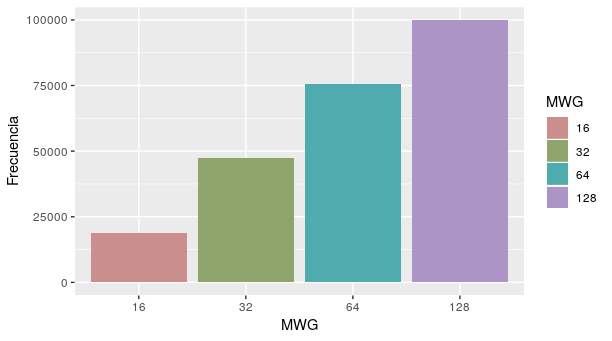
\includegraphics[width=0.45\textwidth]{plots/mwg_bar}
    \caption{Gráfico de barras del atributo $M_{wg}$.}
    \label{figure:mwg_bar}
\end{figure}

\begin{figure}[H]
    \centering
    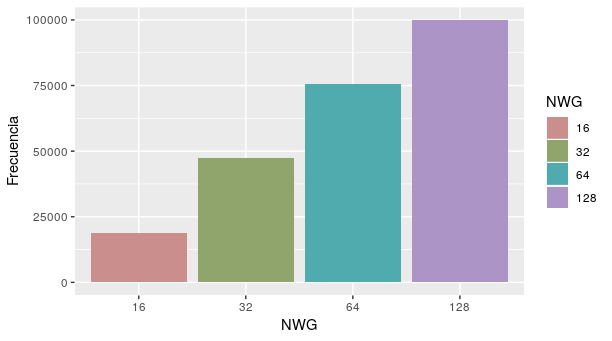
\includegraphics[width=0.45\textwidth]{plots/nwg_bar}
    \caption{Gráfico de barras del atributo $N_{wg}$.}
    \label{figure:nwg_bar}
\end{figure}

\begin{figure}[H]
    \centering
    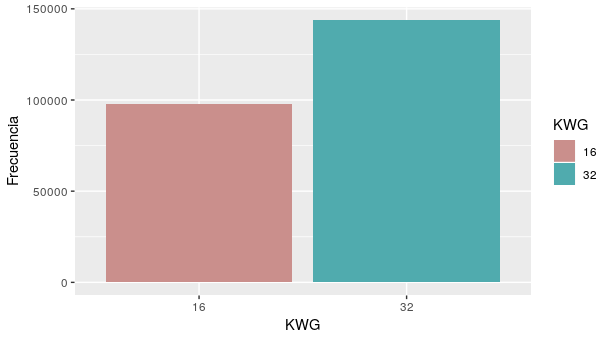
\includegraphics[width=0.45\textwidth]{plots/kwg_bar}
    \caption{Gráfico de barras del atributo $K_{wg}$.}
    \label{figure:kwg_bar}
\end{figure}

\begin{figure}[H]
    \centering
    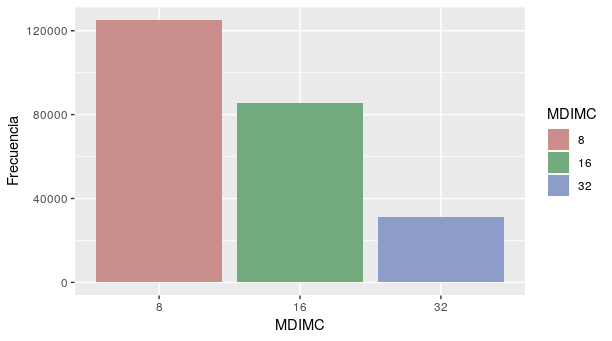
\includegraphics[width=0.45\textwidth]{plots/mdimc_bar}
    \caption{Gráfico de barras del atributo $M_{dim}C$.}
    \label{figure:MDIMC_bar}
\end{figure}

\begin{figure}[H]
    \centering
    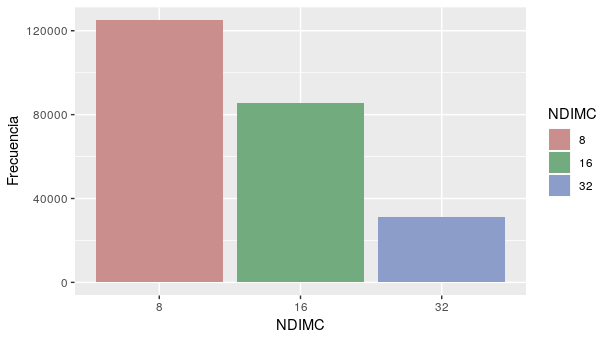
\includegraphics[width=0.45\textwidth]{plots/ndimc_bar}
    \caption{Gráfico de barras del atributo $N_{dim}C$.}
    \label{figure:ndimc_bar}
\end{figure}

\begin{figure}[H]
    \centering
    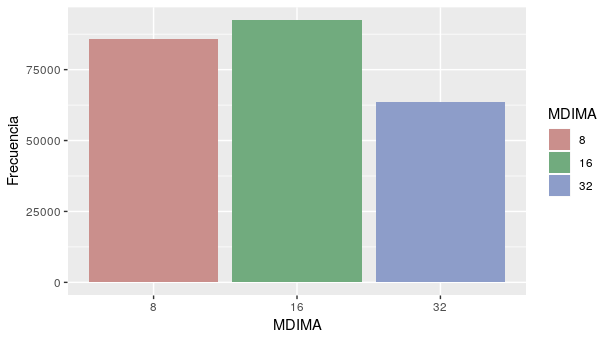
\includegraphics[width=0.45\textwidth]{plots/mdima_bar}
    \caption{Gráfico de barras del atributo $M_{dim}A$.}
    \label{figure:mdima_bar}
\end{figure}

\begin{figure}[H]
    \centering
    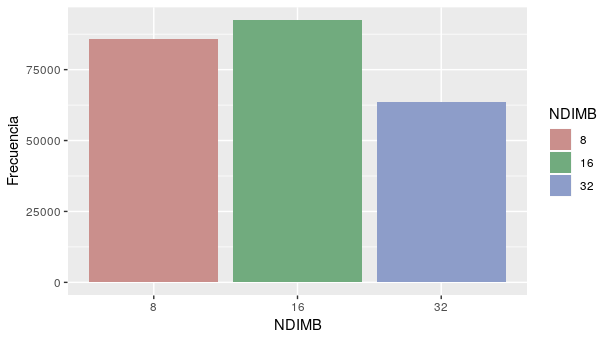
\includegraphics[width=0.45\textwidth]{plots/ndimb_bar}
    \caption{Gráfico de barras del atributo $N_{dim}B$.}
    \label{figure:ndimb_bar}
\end{figure}

\begin{figure}[H]
    \centering
    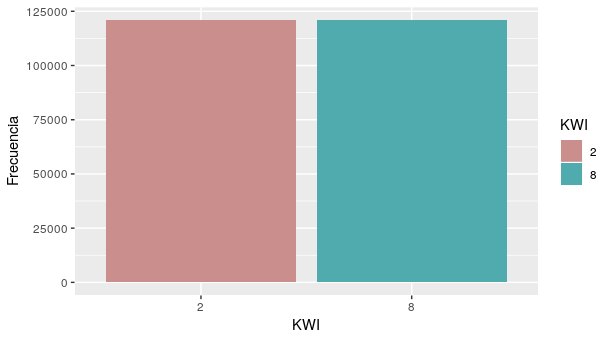
\includegraphics[width=0.45\textwidth]{plots/kwi_bar}
    \caption{Gráfico de barras del atributo $K_{wi}$.}
    \label{figure:kwi_bar}
\end{figure}

\begin{figure}[H]
    \centering
    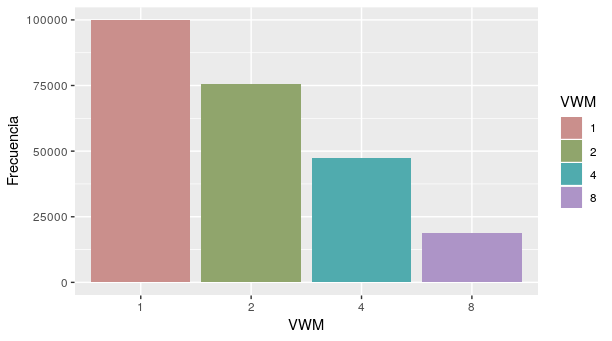
\includegraphics[width=0.45\textwidth]{plots/vwm_bar}
    \caption{Gráfico de barras del atributo $V_{wm}$.}
    \label{figure:vwm_bar}
\end{figure}

\begin{figure}[H]
    \centering
    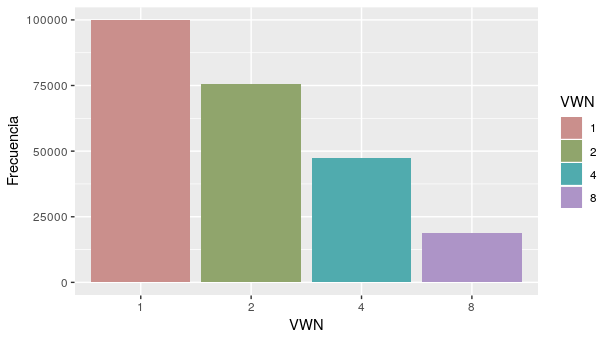
\includegraphics[width=0.45\textwidth]{plots/vwn_bar}
    \caption{Gráfico de barras del atributo $V_{wn}$.}
    \label{figure:vwn_bar}
\end{figure}

\begin{figure}[H]
    \centering
    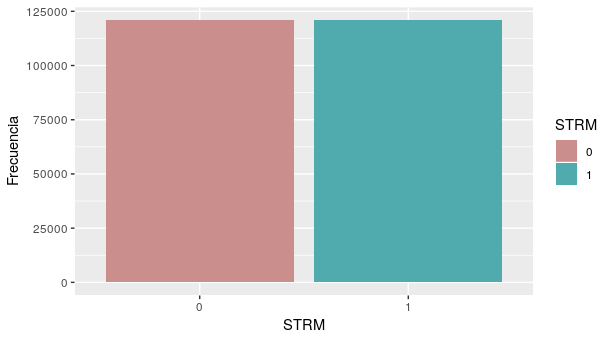
\includegraphics[width=0.45\textwidth]{plots/strm_bar}
    \caption{Gráfico de barras del atributo $M_{stride}$.}
    \label{figure:strm_bar}
\end{figure}

\begin{figure}[H]
    \centering
    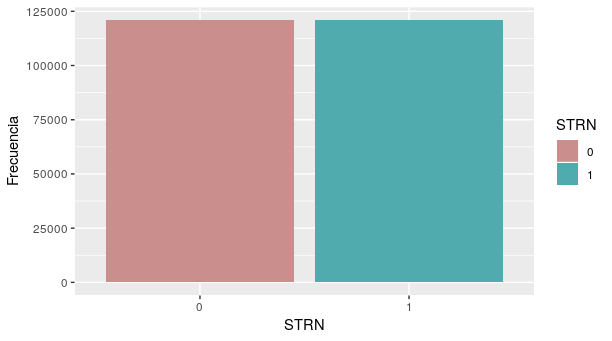
\includegraphics[width=0.45\textwidth]{plots/strn_bar}
    \caption{Gráfico de barras del atributo $N_{stride}$.}
    \label{figure:strn_bar}
\end{figure}

\onecolumngrid

\end{document}
